% =====================================================================================
% Chapter 5 - concise version (v2: ERD figure removed, text shortened where figures carry the detail)
% Required packages in the preamble: graphicx, booktabs, amsmath.
% Figures: copy the folder Demo/docs/figures into the thesis project as figures/.
% \tbd marks values to be filled in after the benchmark is run with all seven checkpoints.
% =====================================================================================
\providecommand{\tbd}{\underline{\hspace{1.2cm}}}

\chapter{System Design and Implementation}
\label{chap:system_design}

This chapter describes how the TriMVPP framework presented in Chapter~4 is realized as an interactive web-based system. It covers the system architecture, the integration of foundation models and bioinformatics resources, the single-variant and batch workflows, data management and deployment, the web interface, and the system's runtime latency.

% -------------------------------------------------------------------------------------
\section{System Architecture}
\label{sec:system_architecture}

The system follows a three-tier client--server architecture (Fig.~\ref{fig:system_architecture}) that separates user interaction, AI orchestration, and data management, so that computationally intensive annotation and inference never block the user interface. The React frontend communicates with a FastAPI backend through REST for single-variant queries and Server-Sent Events (SSE) for streaming batch results. The backend orchestrates the complete inference workflow and runs blocking operations, such as VEP annotation and GPU computation, in background threads. All data resources, including the PostgreSQL database and the bioinformatics references, are deployed locally, which ensures reproducible annotation and removes any dependence on external web services.

\begin{figure}[htbp]
    \centering
    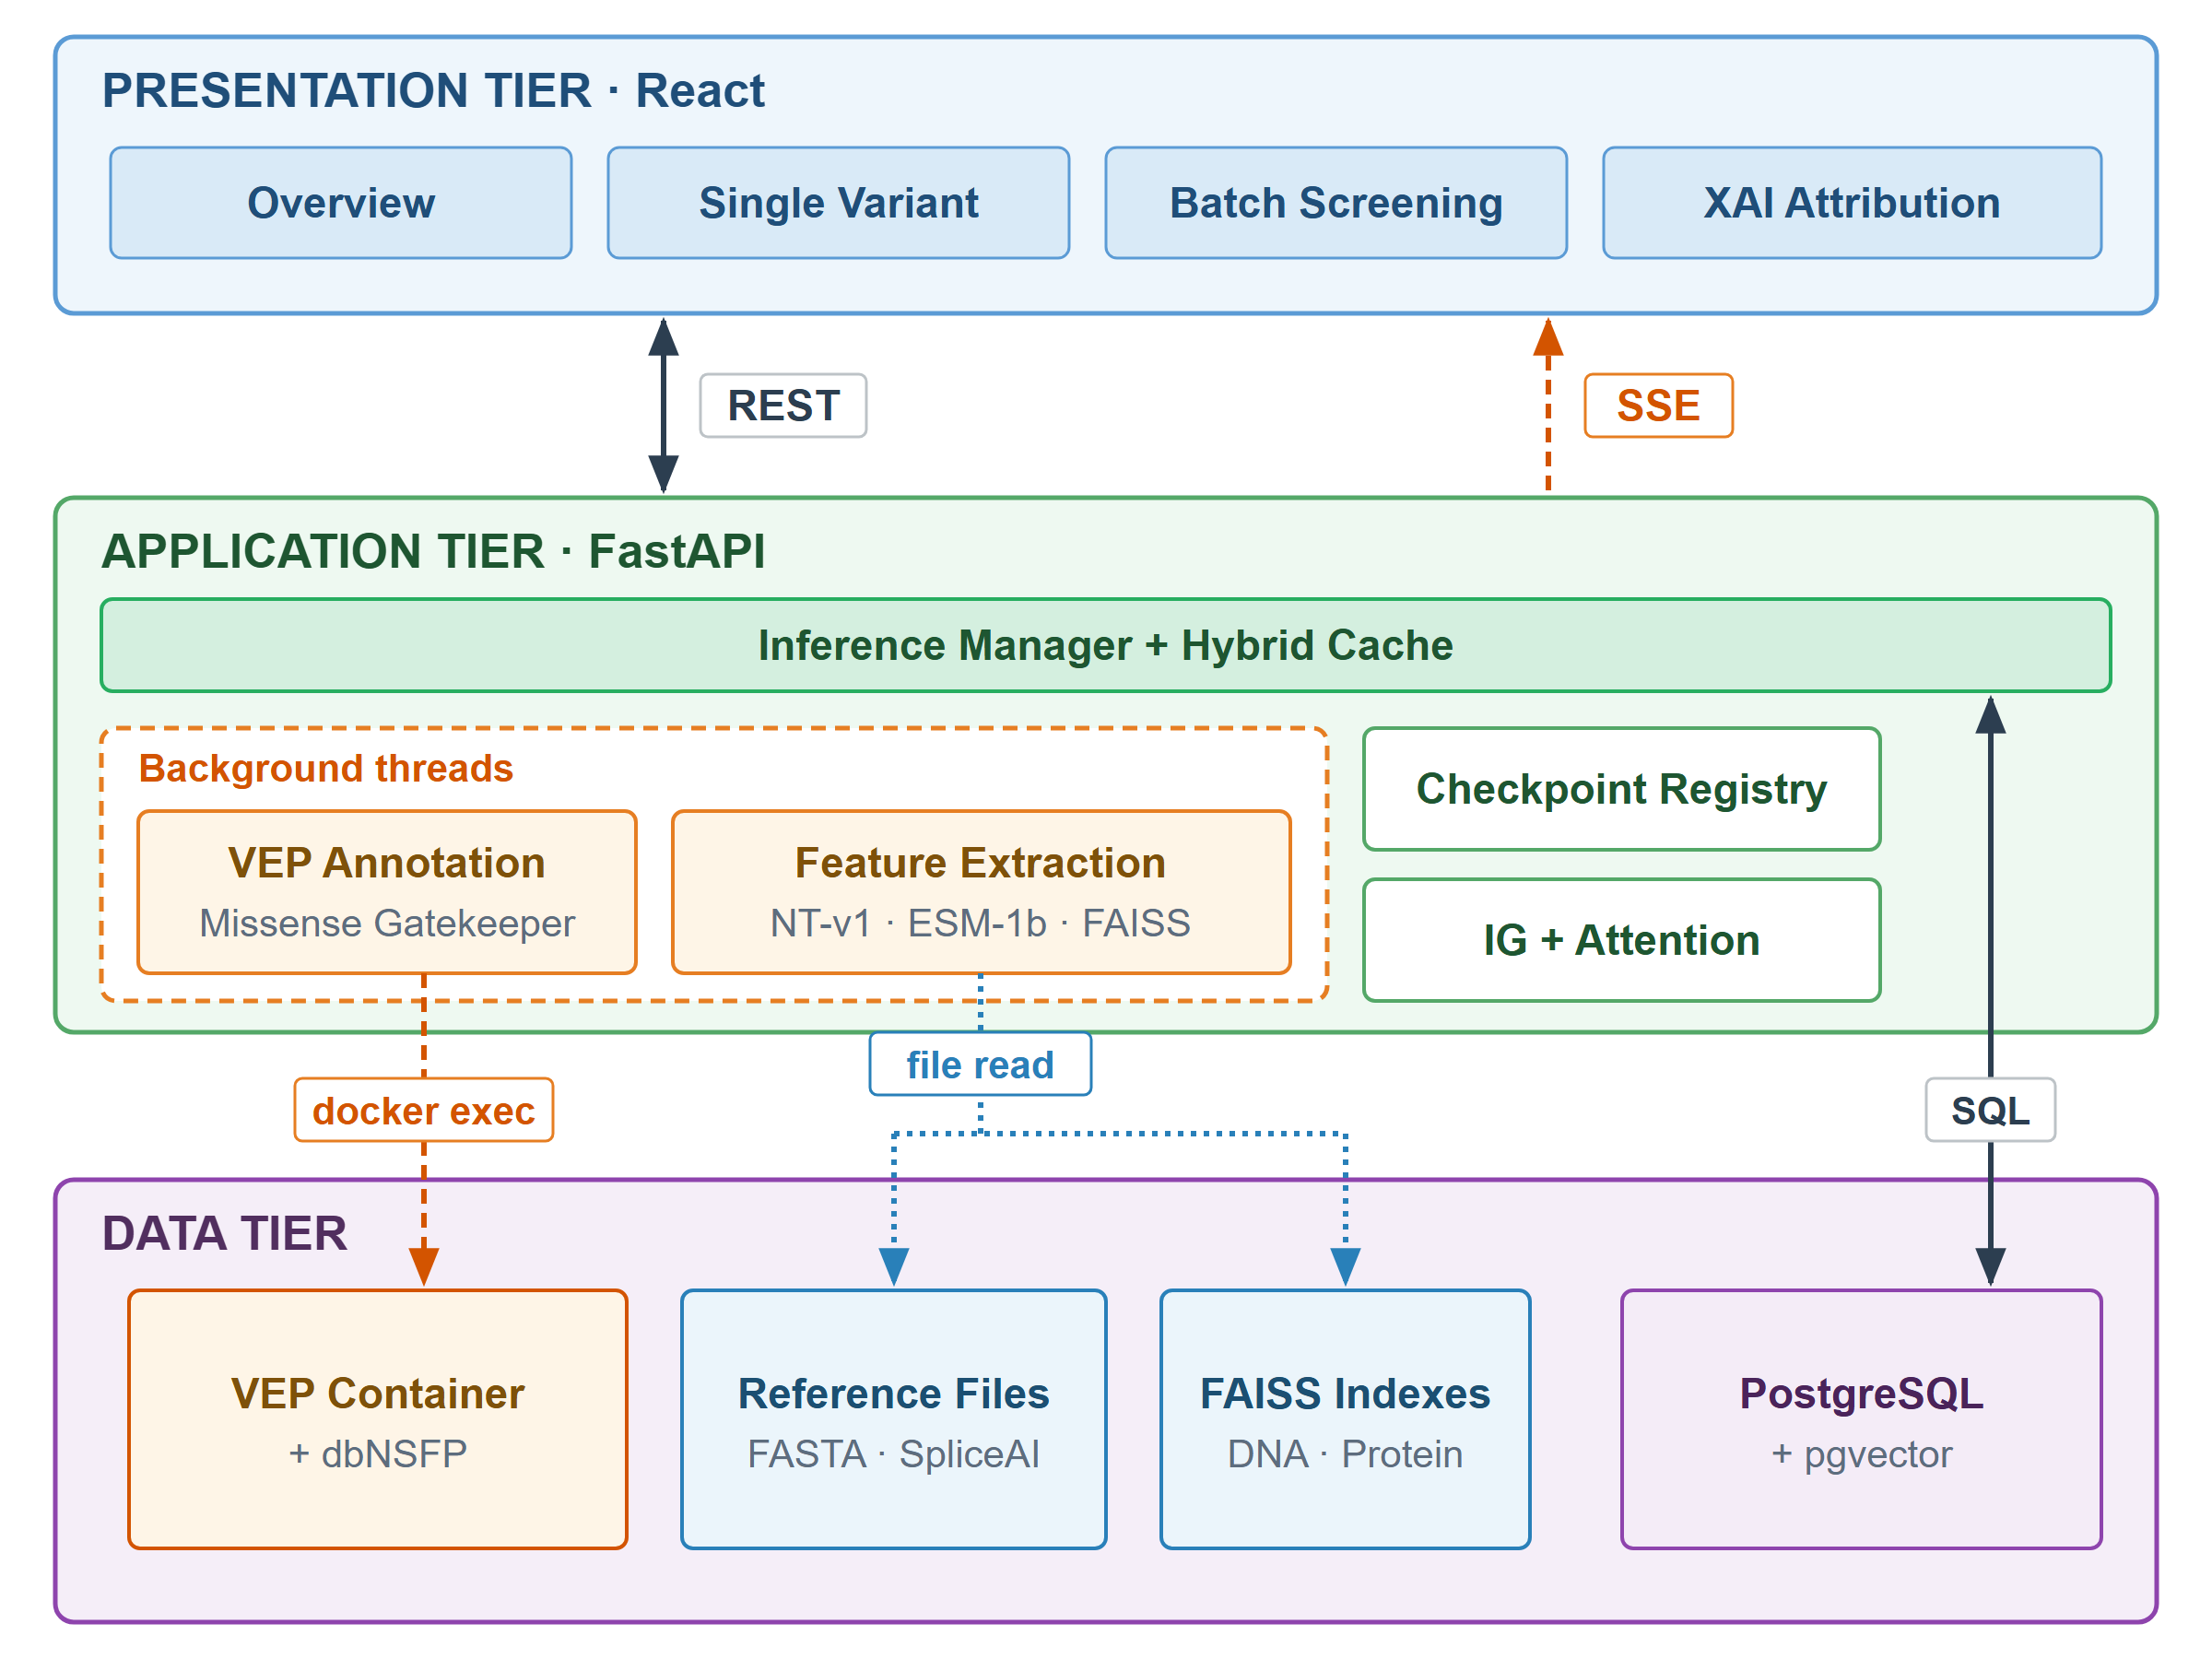
\includegraphics[width=0.95\textwidth]{figures/5.1.png}
    \caption{Three-tier architecture of the TriMVPP system.}
    \label{fig:system_architecture}
\end{figure}

% -------------------------------------------------------------------------------------
\section{Artificial Intelligence Model and Bioinformatics Integration}
\label{sec:ai_integration}

\subsection{Feature Extraction Pipeline}

To avoid cold-start latency, the backend loads the foundation models, sequence and FAISS indexes, and normalization artifacts once at startup and performs a warm-up forward pass before accepting requests. Each variant, specified as \texttt{chr:pos:ref>alt} on GRCh38, is annotated by the offline Ensembl VEP service, which selects the MANE Select or canonical transcript and provides the consequence, the protein position, and the eleven core biological features: two population allele frequencies from the VEP cache and nine conservation scores from dbNSFP. AlphaMissense, REVEL, and ClinVar annotations are retrieved at the same time for benchmarking.

Since TriMVPP is trained exclusively on missense single-nucleotide variants, a missense gatekeeper rejects every other consequence type, and the reference allele and amino acid are verified against the local GRCh38 genome and proteome to detect inputs from an incorrect genome build. For accepted variants, the nine SpliceAI features are read from the compressed SpliceAI archive through a custom tabix reader that decompresses only the blocks surrounding the variant. The DNA and protein windows ($1{,}001$~bp and $501$~aa) centered on the mutation are encoded by NT-v1 500M\footnote{\url{https://huggingface.co/InstaDeepAI/nucleotide-transformer-500m-human-ref}} and ESM-1b 650M\footnote{\url{https://huggingface.co/facebook/esm1b_t33_650M_UR50S}} in FP32 precision, and the resulting embeddings are used to compute the geometric descriptors, including the local intrinsic dimensionality estimated from $k = 64$ nearest neighbors in the FAISS indexes.

\subsection{Ablation-Aware Model Routing}

The web interface exposes three feature groups, each controlled by a single switch: \textit{DNA}, \textit{Protein}, and \textit{Bio + Geom + SpliceAI}. Since disabling all groups is not allowed, the system supports seven configurations (Table~\ref{tab:ablation_configs}). A checkpoint registry maps each configuration to its trained checkpoint and infers the architecture directly from the stored weights, so that new checkpoints can be activated without code changes. The full configuration uses the \texttt{RouterExpertCorrection} model ($6{,}462{,}728$ parameters, router temperature $T = 0.3074$, learnable correction weight $\beta$), while the six reduced configurations use \texttt{MultiStrategyFusionModel} checkpoints. Each checkpoint applies its own MCC-optimal threshold $\tau$ (e.g., $\tau = 0.6376$ for the full configuration), and a variant is classified as \textit{Pathogenic} if $p \geq \tau$.

\begin{table}[htbp]
    \centering
    \caption{Feature-ablation configurations supported by the checkpoint registry.}
    \label{tab:ablation_configs}
    \begin{tabular}{clcc}
        \toprule
        \textbf{Key} & \textbf{Active feature groups} & \textbf{Architecture} & \textbf{SHAP players} \\
        \midrule
        \texttt{111} & DNA, Protein, Bio + Geom + SpliceAI & RouterExpertCorrection & 30 \\
        \texttt{110} & DNA, Protein & MultiStrategyFusion & 2 \\
        \texttt{101} & DNA, Bio + Geom + SpliceAI & MultiStrategyFusion & 29 \\
        \texttt{011} & Protein, Bio + Geom + SpliceAI & MultiStrategyFusion & 29 \\
        \texttt{100} & DNA & MultiStrategyFusion & 1 \\
        \texttt{010} & Protein & MultiStrategyFusion & 1 \\
        \texttt{001} & Bio + Geom + SpliceAI & MultiStrategyFusion & 28 \\
        \bottomrule
    \end{tabular}
\end{table}

\subsection{Integrated Explainability}

Instead of relying on an external explainability library, the inference engine embeds a GPU-based permutation Shapley estimator. Each active embedding displacement ($\boldsymbol{\delta}_{\text{DNA}}$ or $\boldsymbol{\delta}_{\text{Prot}}$) is treated as one player and each of the $28$ standardized tabular features as an individual player, giving $n = 30$ players for the full configuration. Using a zero baseline, the engine samples $128$ antithetic permutations, evaluates all $128 \times (n + 1)$ nested coalitions as one batched tensor ($3{,}968$ forward passes for the full configuration), and returns logit-scale attributions satisfying the efficiency property
\[
    \sum_{i=1}^{n} \phi_i = f(\mathbf{x}) - f(\mathbf{0}).
\]
Because the attributions are computed in the same request, every prediction is accompanied by its feature-level explanation.

% -------------------------------------------------------------------------------------
\section{Data Flow and Communication Protocols}
\label{sec:data_flow}

\subsection{Single-Variant Inference with Hybrid Lazy-Caching}

To keep interactive exploration fast, the system caches upstream features and downstream predictions separately, so that each request follows one of the three paths in Fig.~\ref{fig:single_sequence}. A \textit{cache hit} returns a stored prediction directly. A \textit{feature reuse}, triggered by a configuration change or \textit{Live Bypass} mode, reloads the stored features and re-executes only classification and explanation. A \textit{cache miss} runs the full pipeline, in which the slow VEP annotation is overlapped with the DNA feature extraction, and the upstream features are persisted before classification so that a later failure never forces the costly extraction to be repeated. Cached entries carry a fingerprint of the extraction settings and the checkpoint identity, so that any change to the pipeline or the model automatically invalidates outdated results.

\begin{figure}[htbp]
    \centering
    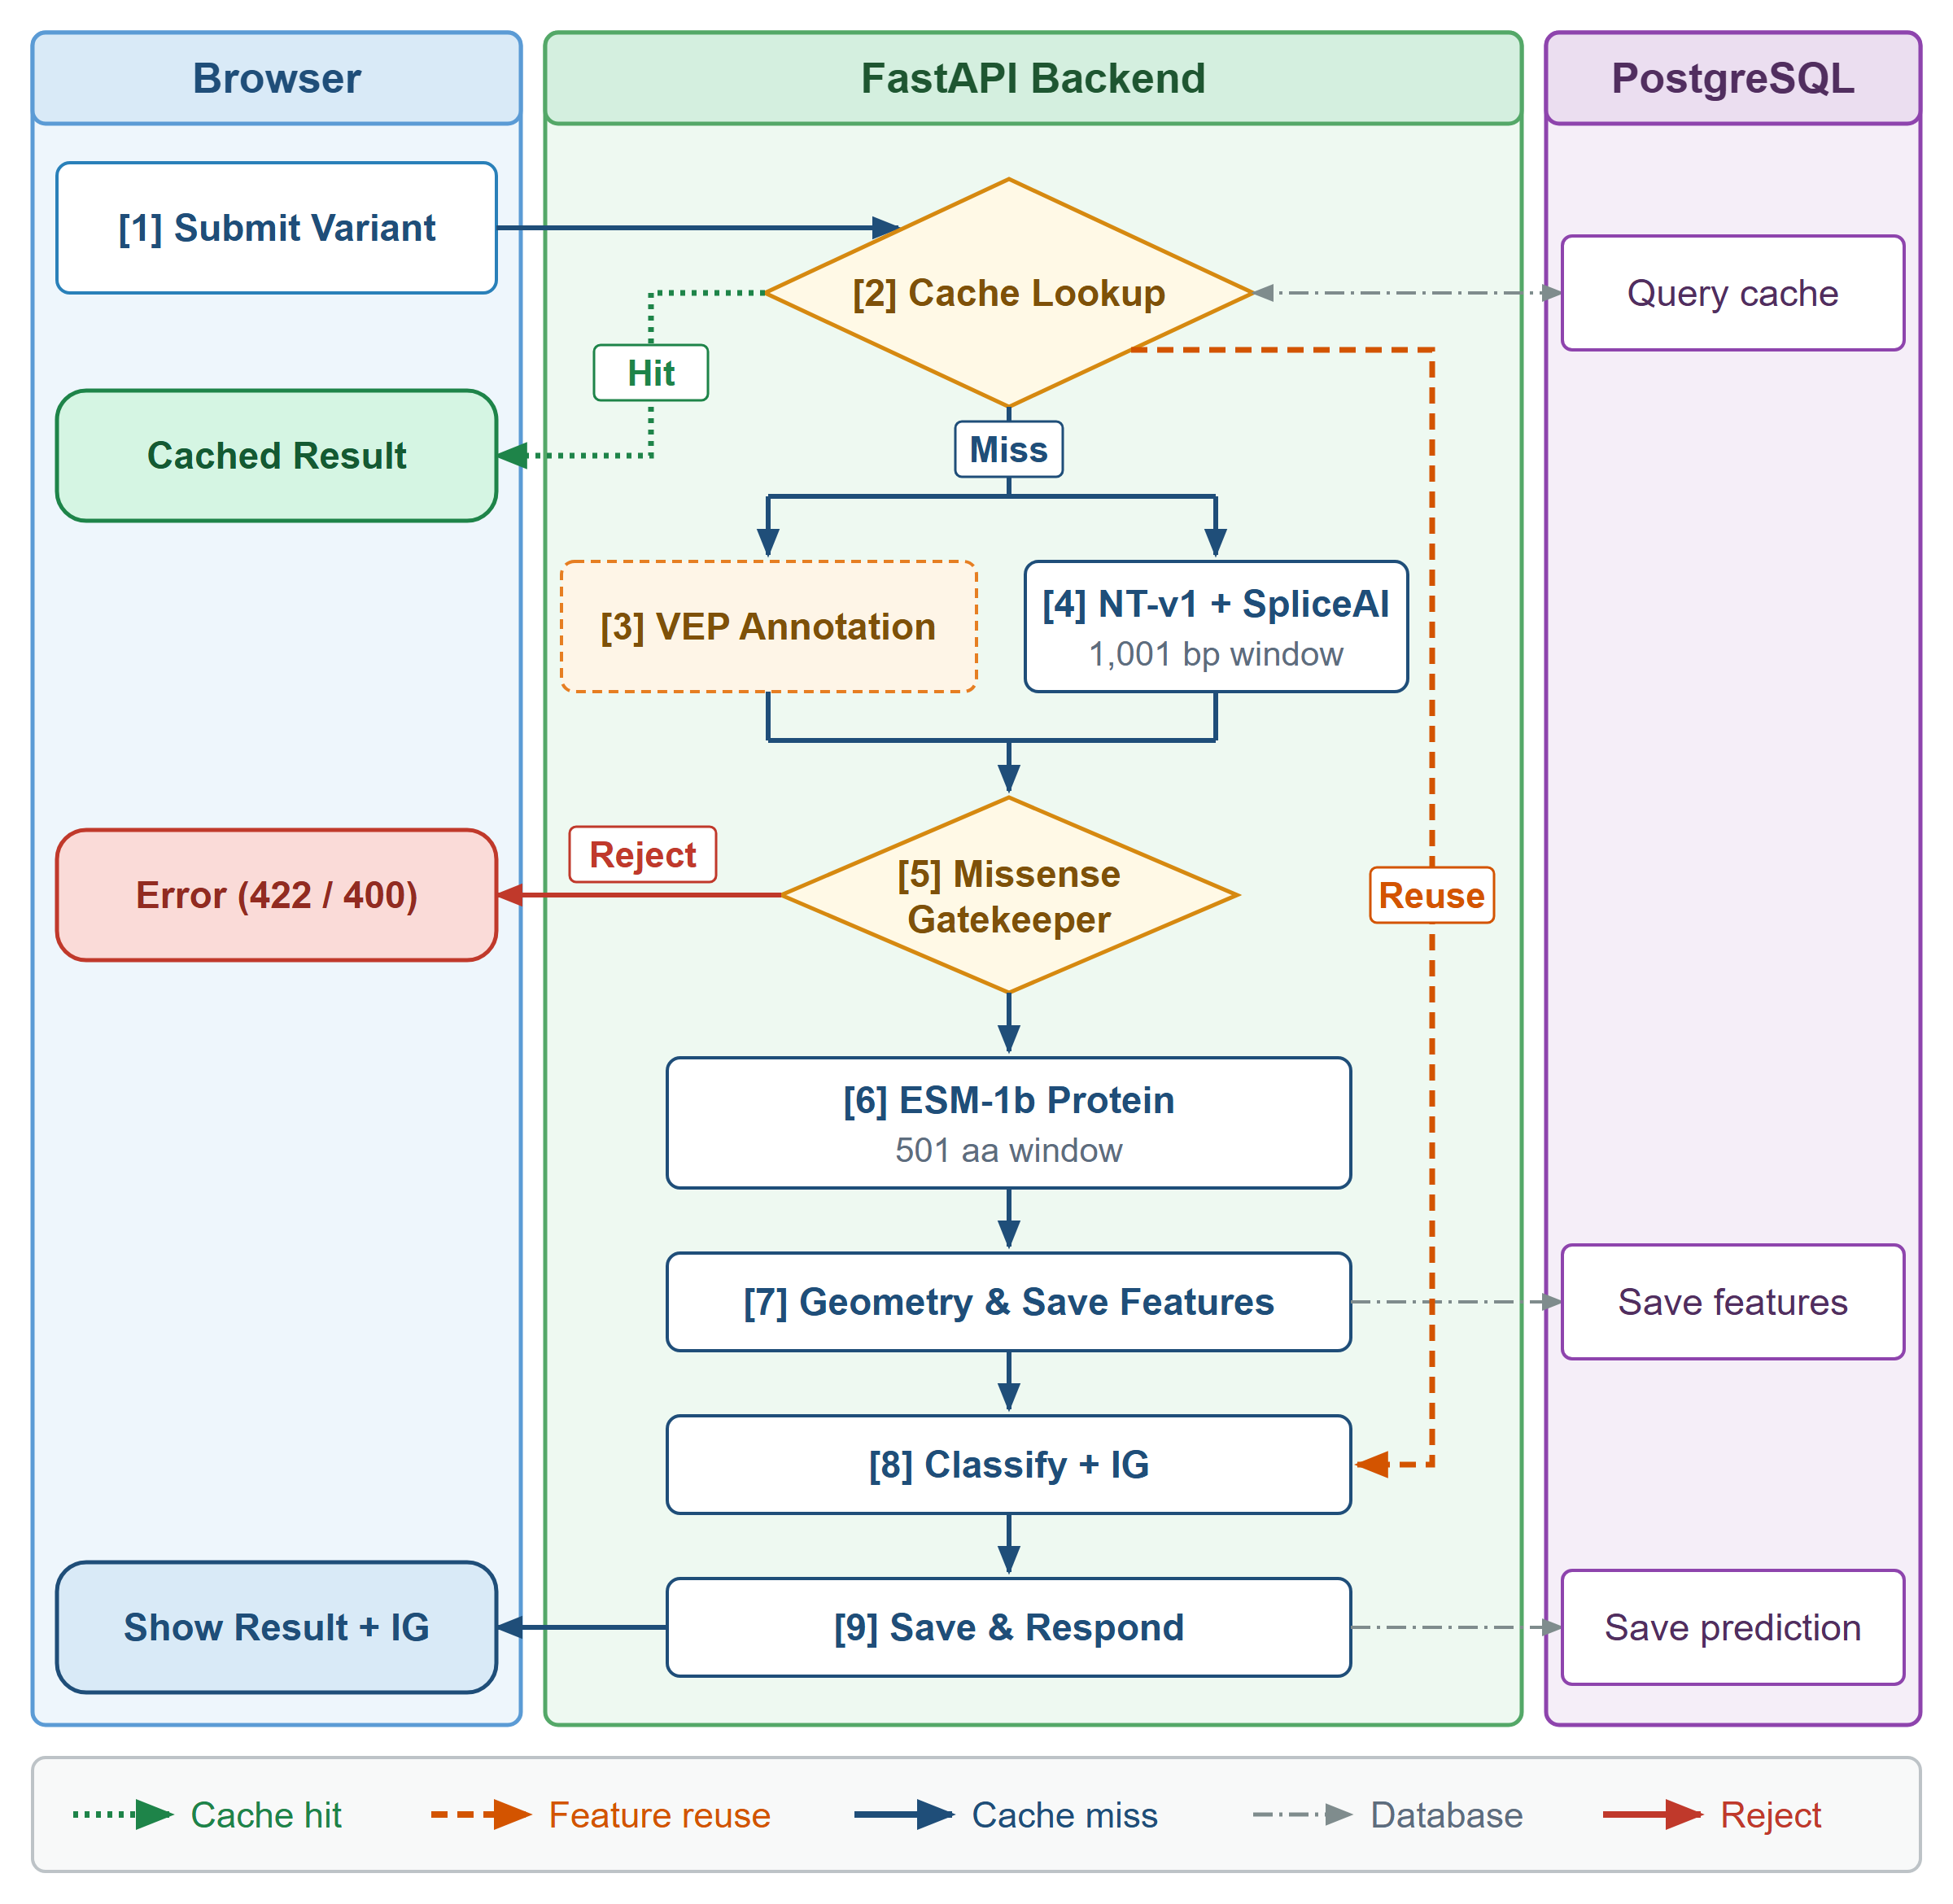
\includegraphics[width=0.95\textwidth]{figures/5.2.png}
    \caption{Single-variant inference workflow with hybrid lazy-caching.}
    \label{fig:single_sequence}
\end{figure}

\subsection{Batch Screening via Server-Sent Events}

Batch screening (Fig.~\ref{fig:batch_sse}) accepts a variant file (VCF, CSV, TXT, Parquet, or Excel) or a built-in $10$-variant benchmark cohort and streams results through SSE, which avoids HTTP timeouts and shows progress in real time. All uncached variants are annotated in a single VEP run, and the accepted variants are encoded in micro-batches of up to eight variants per foundation model forward pass. Each variant's result is emitted as soon as it is classified, so the browser's triage table fills incrementally instead of waiting for the whole cohort.

\begin{figure}[htbp]
    \centering
    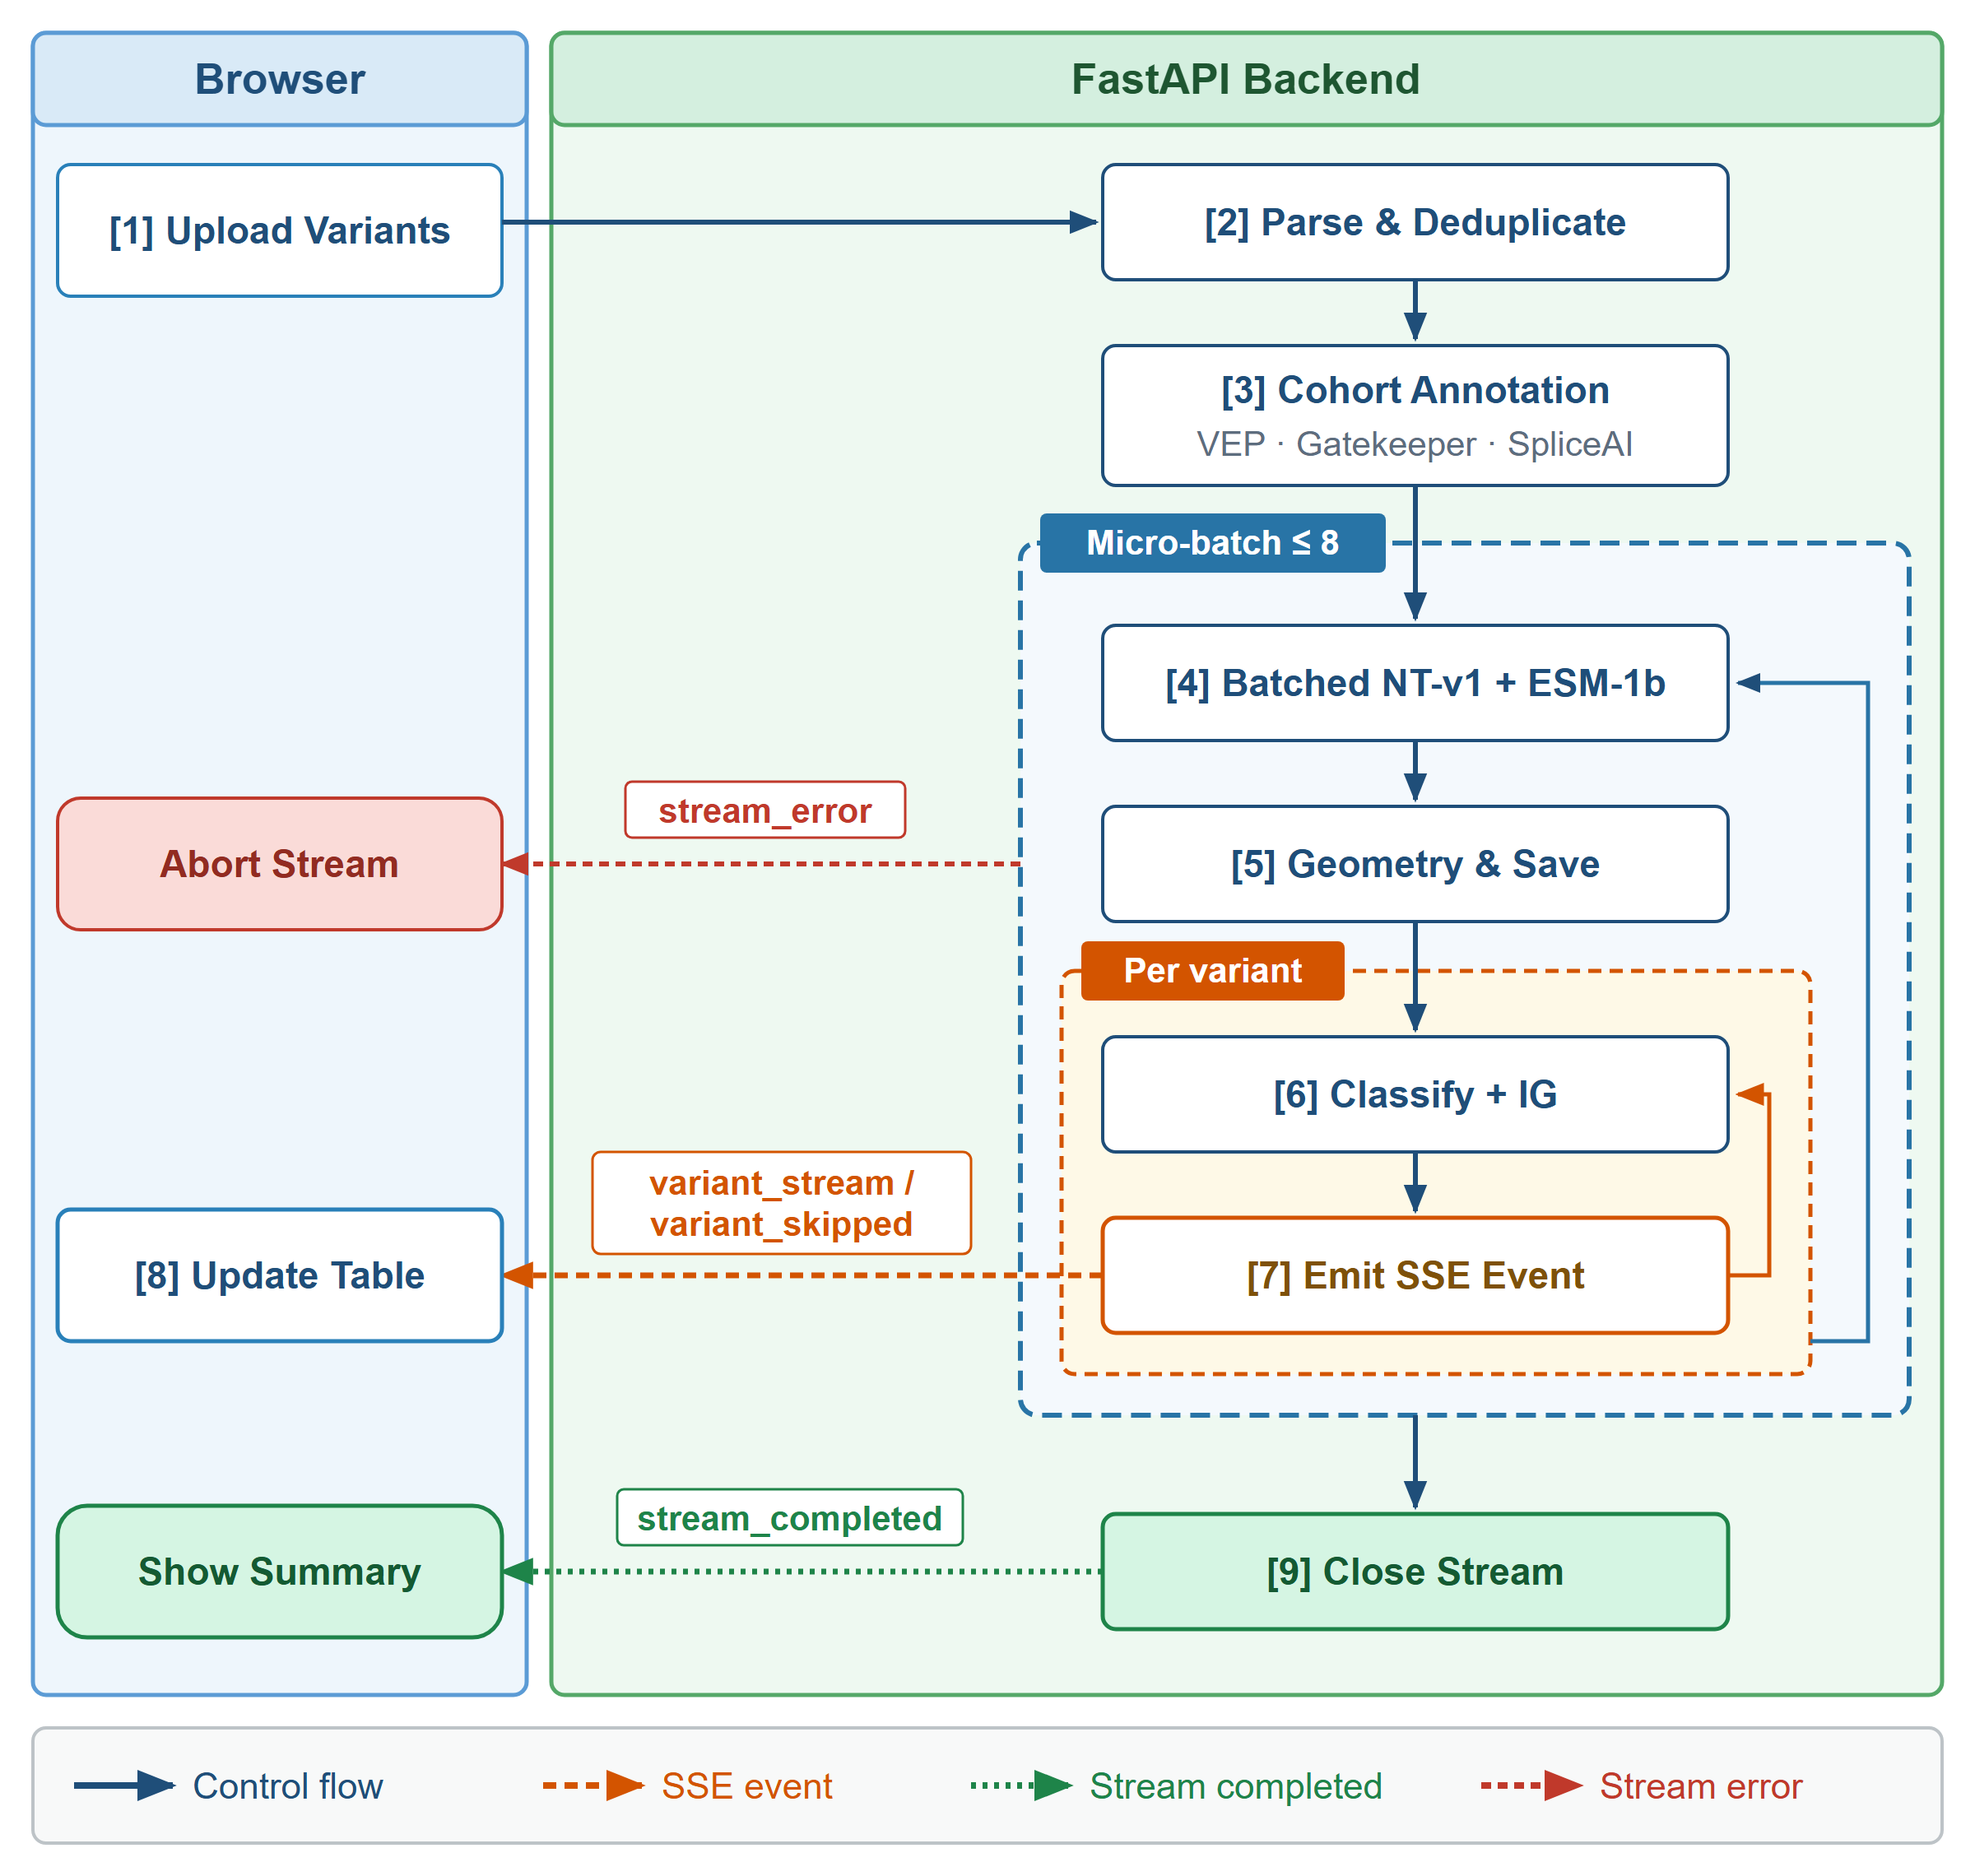
\includegraphics[width=0.95\textwidth]{figures/5.3.png}
    \caption{Batch screening workflow with micro-batched inference and SSE streaming.}
    \label{fig:batch_sse}
\end{figure}

% -------------------------------------------------------------------------------------
\section{Data Management and Deployment}
\label{sec:db_deployment}

The PostgreSQL database consists of three tables. The \texttt{variants} table stores each GRCh38 variant with its gene, consequence, protein change, and normalized ClinVar label. The \texttt{inference\_features} table keeps one record per variant with the four $1{,}280$-dimensional reference and alternative embeddings as \texttt{pgvector} columns, the unscaled biological and geometric features, and the extraction fingerprint; the embeddings are rounded to FP16 precision before storage to match the format used during training. The \texttt{predictions} table holds at most one record per variant and feature configuration, containing the probability, label, benchmark scores, Shapley attributions, and model version. All writes are atomic upserts.

The system adopts a hybrid deployment: PostgreSQL and the offline VEP service run in Docker containers, which isolates their dependencies, whereas the FastAPI backend runs natively to obtain direct access to the CUDA runtime and loads the foundation models on the GPU only once at startup. A single startup script launches the database, backend, and frontend. The main technologies are summarized in Table~\ref{tab:tech_stack}.

\begin{table}[htbp]
    \centering
    \caption{Technology stack of the TriMVPP system.}
    \label{tab:tech_stack}
    \begin{tabular}{ll}
        \toprule
        \textbf{Layer} & \textbf{Technologies} \\
        \midrule
        Frontend & React 19, TypeScript, Vite, Tailwind CSS, Recharts \\
        Backend & Python 3.10, FastAPI, Uvicorn, Pydantic, SQLAlchemy \\
        Deep learning & PyTorch 2.4 (CUDA 12.1), Hugging Face Transformers, FAISS \\
        Database & PostgreSQL 16 with \texttt{pgvector} (Docker) \\
        Bioinformatics & Ensembl VEP 116 with dbNSFP 5.3.1a (Docker), SpliceAI MANE v1.4, pyfaidx \\
        \bottomrule
    \end{tabular}
\end{table}

% -------------------------------------------------------------------------------------
\section{Web Interface}
\label{sec:web_interface}

The web interface (Fig.~\ref{fig:web_interface}) provides four views. The overview page (a) introduces the system and links to each module. The single-variant view (b) accepts a GRCh38 coordinate and the three feature switches, and displays the predicted probability and label alongside ClinVar, AlphaMissense, and REVEL; a \textit{Live Bypass} option forces recomputation. The batch view (c) shows the streaming progress, the numbers of accepted and rejected variants, and a live triage table of the most likely pathogenic variants. The explainability view (d) presents the Shapley attributions of a selected variant as a diverging bar chart. Results can be opened across views with their variant and feature configuration preserved.

\begin{figure}[htbp]
    \centering
    % Replace each box with \includegraphics[width=\linewidth]{figures/5.4x.png}
    \begin{minipage}{0.48\textwidth}\centering
        \fbox{\parbox{0.95\linewidth}{\centering\vspace{1.6cm}\textit{[Overview page]}\vspace{1.6cm}}}\\[2pt]
        \small (a) System overview
    \end{minipage}\hfill
    \begin{minipage}{0.48\textwidth}\centering
        \fbox{\parbox{0.95\linewidth}{\centering\vspace{1.6cm}\textit{[Single-variant view]}\vspace{1.6cm}}}\\[2pt]
        \small (b) Single-variant inspection
    \end{minipage}\\[8pt]
    \begin{minipage}{0.48\textwidth}\centering
        \fbox{\parbox{0.95\linewidth}{\centering\vspace{1.6cm}\textit{[Batch view]}\vspace{1.6cm}}}\\[2pt]
        \small (c) Batch screening
    \end{minipage}\hfill
    \begin{minipage}{0.48\textwidth}\centering
        \fbox{\parbox{0.95\linewidth}{\centering\vspace{1.6cm}\textit{[Explainability view]}\vspace{1.6cm}}}\\[2pt]
        \small (d) Explainability analysis
    \end{minipage}
    \caption{Main views of the TriMVPP web interface.}
    \label{fig:web_interface}
\end{figure}

% -------------------------------------------------------------------------------------
\section{Latency Evaluation}
\label{sec:latency}

Runtime latency was measured on a workstation with an AMD Ryzen~7 8745H CPU, 32~GB of RAM, and an NVIDIA GeForce RTX 4060 Laptop GPU (8~GB VRAM) running Windows~11, with all inference in FP32. Startup preloading takes approximately \tbd{}~s and \tbd{}~GB of GPU memory and is excluded from the measurements. % TODO: fill in after the FP32 benchmark
Latency was recorded by the backend profiler, from request entry until the response is constructed, under a sequential single-user workload on the $10$-variant benchmark cohort (Table~\ref{tab:latency_benchmarks}).

% TODO: fill in the latency column once all seven checkpoints are available.
\begin{table}[htbp]
    \centering
    \caption{Server-side processing latency across execution paths on the reference workstation.}
    \label{tab:latency_benchmarks}
    \begin{tabular}{llr}
        \toprule
        \textbf{Scenario} & \textbf{Execution path} & \textbf{Latency} \\
        \midrule
        Single new variant & Full cache miss & \tbd{} s / variant \\
        Batch cohort ($10$ variants) & Full cache miss & \tbd{} s total \\
        Configuration change / Live Bypass & Feature reuse & \tbd{} s / query \\
        Repeated query & Full cache hit & \tbd{} ms / query \\
        \bottomrule
    \end{tabular}
\end{table}

Batch processing reduces the average cost to \tbd{}~s per variant, a \tbd{}$\times$ speed-up over sequential single-variant requests, mainly because VEP is invoked once for the whole cohort and the foundation models process several variants per forward pass. Once a variant's features are stored, changing the feature configuration takes only \tbd{}~s, and repeated queries are answered in \tbd{}~ms, enabling responsive interactive exploration.
